%% This is an example first chapter.  You should put chapter/appendix that you
%% write into a separate file, and add a line \include{yourfilename} to
%% main.tex, where `yourfilename.tex' is the name of the chapter/appendix file.
%% You can process specific files by typing their names in at the
%% \files=
%% prompt when you run the file main.tex through LaTeX.
\chapter{Motivation and Examples}
\label{chap:motivation}

Understanding elementary geometry is a fundamental reasoning skill,
and encompasses a domain both constrained enough to model effectively,
yet rich enough to allow for interesting insights.  Although
elementary geometry knowledge can be conveyed via series of factual
definitions, theorems, and proofs, a particularly intriguing aspect of
geometry is the ability for students to learn and develop an
understanding of core concepts through visual investigation,
exploration, and discovery.

These visual reasoning skills reflect many of the cognitive activities
used as one interacts with his or her surroundings.  Day-to-day
decisions regularly rely on visual reasoning processes such as
imagining what three dimensional objects look like from other angles,
or mentally simulating the effects of one's actions on objects based
on a learned understanding of physics and the object's properties.
Such skills and inferred rules are developed through repeated
observation, followed by the formation and evaluation of conjectures.

Similar to such day-to-day three-dimensional reasoning, visualizing
and manipulating 2D geometric diagrams ``in the mind's eye'' allows
one to explore questions such as ``what happens if...''  or ``is it
always true that...''  to discover new conjectures.  Further
investigation of examples can increase one's belief in such a
conjecture, and an accompanying system of deductive reasoning from
basic axioms could prove that an observation is correct.

As an example, a curious student might notice that in a certain
drawing of a triangle, the three perpendicular bisectors of the edges
are concurrent, and that a circle constructed with center at the point
of concurrence intersects all three vertices of the triangle.  Given
this ``interesting observation,'' the student might explore other
triangles to see if this behavior is just coincidence, or conjecture
about whether it applies to certain classes of triangles or all
triangles in general.  After investigating several other examples, the
student might have sufficient belief in the conjecture to explore
using previously-proven theorems (in this case, correspondences in
congruent triangles) to prove the conjecture.  My proposed project is
a software system that simulates and automates this inductive thought
process.

Automating geometric reasoning is not new, and has been an active
field in computing and artificial intelligence.  Dynamic geometry
software, automated proof assistants, deductive databases, and several
reformulations into abstract algebra models have been proposed in the
last few decades.  Although many of these projects have focused on the
end goal of obtaining rigorous proofs of geometric theorems, I am
particularly interested in exploring and modeling the more creative
human-like thought processes of inductively exploring and manipulating
diagrams to \emph{discover} new insights about geometry.

I propose the creation and analysis of an interactive computer system
that emulates the curious student described above, and is capable of
exploring geometric concepts through inductive investigation.  The
system will begin with a fairly limited set of factual knowledge
regarding basic definitions in geometry and provide means by which a
user interacting with the system could ``teach'' the system additional
geometric concepts and theorems by suggesting investigations the
system should explore to see if it ``notices anything interesting.''

To evaluate its recognition of such concepts, the interactive system
will provide means for a user to extract the observations and apply
its findings to new scenarios.  In addition to the automated reasoning
and symbolic artificial intelligence aspects of a system that can
learn and reason inductively about geometry, the project also has some
interesting opportunities to explore educational concepts related to
experiential learning, and several extensions to integrate it with
existing construction synthesis and proof systems.

\section{Manipulating Diagrams ``In the Mind's Eye''}

Although the field of mathematics has developed a rigorous structure
of deductive proofs explaining most findings in geometry, much of
human intuition and initial reasoning about geometric ideas come not
from applying formal rules, but rather from visually manipulating
diagrams ``in the mind's eye.''


\subsection{An Initial Example}

\begin{center}
\includegraphics[width=0.80\textwidth]{diagrams/rectangles.eps}
\end{center}

\noindent {\bf Example 1: Of the three diagrams above, determine which
  have constraints sufficient to restrict the quadrilateral $ABCD$ to
  always be a rectangle.}

An automated deductive solution to this question could attempt to use
forward-chaining of known theorems to determine whether there was a
logical path that led from the given constraints to the desired result
that the quadrilateral shown is a rectangle.  However, getting the
correct results would require having a rich enough set of inference
rules and a valid system of applying them.

A more intuitive visual-reasoning approach usually first explored by
humans is to initially verify that the marked constraints hold for the
instance of the diagram as drawn and then mentally manipulate or
``wiggle'' the diagram to see if one can find a nearby counter-example
that still satisfies the given constraints, but is not a rectangle.
If the viewer is unable to find a counter-example after several
attempts, he or she may be sufficiently convinced the conclusion is
true, and could commit to exploring a more rigorous deductive proof.

\begin{center}
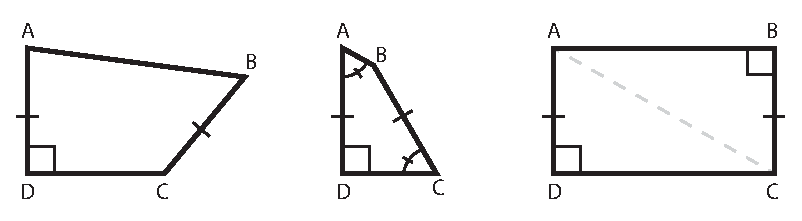
\includegraphics[width=0.80\textwidth]{diagrams/rectangles-answer.eps}
\end{center}

\noindent {\bf Solution to Example 1: As the reader likely discovered,
  the first two diagrams can be manipulated to yield instances that
  are not rectangles, while the third is sufficiently constrained to
  always represent a rectangle.  (This can be proved by adding a
  diagonal and using the Pythagorean theorem.)}

\subsection{Diagrams, Figures, and Constraints}

This example of manipulation using the ``mind's eye'' also introduces
some terminology helpful in discussing the differences between images
as drawn and the spaces of geometric objects they represent.  For
clarity, a \emph{figure} will refer to an actual configuration of
points, lines, and circles drawn on a page.  Constraint annotations
(congruence or measure) added to a figure create a \emph{diagram},
which represents the entire space of figure \emph{instances} that
satisfy the constraints.

An annotated figure presented on a page is typically an instance of
its corresponding diagram.  However, it is certainly possible to add
annotations to a figure that are not satisfied by that figure,
yielding impossible diagrams.  In such a case the diagram represents
an empty set of satisfying figures.

In the initial example above, the three quadrilaterals figures are
drawn as rectangles.  It is true that all quadrilateral figures in the
space represented by the third diagram are rectangles.  However, the
space of quadrilaterals represented by the first two diagrams include
instances that are not rectangles, as shown above.  At this time, we
will only start with valid diagrams whose constraints are satisfied in
the given figure.  However, detecting and explaining inconsistent
diagrams could be an interesting extension.

\section{Geometry Investigation}

These same ``mind's eye'' reasoning techniques can be used to discover
and learn new geometric theorems.  Given some ``interesting
properties'' in a particular figure, one can construct other instances
of the diagram to examine if the properties appear to hold uniformly,
or if they were just coincidences in the initial drawing.  Properties
that are satisfied repeatedly can be further explored and proved using
deductive reasoning.  The examples below provide several
demonstrations of such inductive investigations.

\subsection{Vertical Angles}

\begin{center}
\includegraphics[width=0.9\textwidth]{diagrams/vertical.eps}
\end{center}

\noindent {\bf Investigation 1: Construct a pair of vertical angles.
  Notice anything interesting?}

Often one of the first theorems in a geometry course, the fact that
vertical angles are equal is one of the simplest examples of applying
``mind's eye'' visual reasoning.  Given the diagram on the left, one
could ``wiggle'' the two lines in his or her mind and imagine how the
angles respond.  In doing so, one would notice that the lower angle's
measure increases and decreases proportionately with that of the top
angle.  This mental simulation, perhaps accompanied by a few drawn and
measured figures, could sufficiently convince the viewer that vertical
angles always have equal measure.

Of course, this fact can also be proved deductively by adding up pairs
of angles that sum to 180 degrees.  However, the inductive
manipulations are more reflective of the initial, intuitive process
one typically takes when first presented with understanding a diagram.

\subsection{Elementary Results}
\label{sec:elem}

\begin{center}
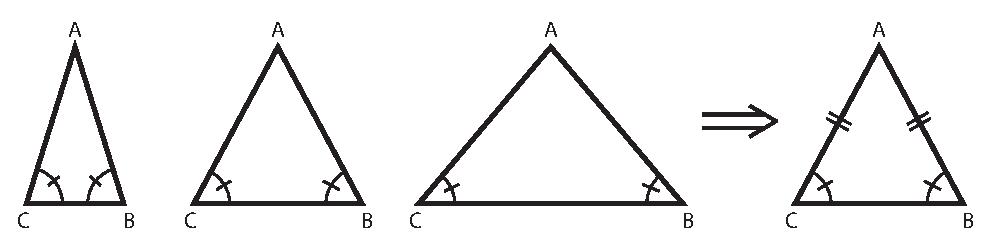
\includegraphics[width=0.9\textwidth]{diagrams/isoceles-triangle.eps}
\end{center}

\noindent {\bf Investigation 2: Construct a triangle $ABC$ with
  $\angle B = \angle C$.  Notice anything interesting?}

A slightly more involved example includes discovering that if a
triangle has two congruent angles, it is isoceles.  As above, this
fact has a more rigorous proof that involves dropping an altitude from
point $A$ and using corresponding parts of congruent triangles to
demonstrate the equality of $AB$ and $AC$.  However, the inductive
investigation of figures that satisfy the constraints can yield the
same conjecture, give students better intuition for what is happening,
and help guide the discovery and assembly of known rules to be applied
in future situations.

In this and further examples, an important question becomes what
properties are considered ``interesting'' and worth investigating in
further instances of the diagram, as discussed in section
\ref{sec:interest}.  As suggested by the examples in Investigation 3,
this can include relations between segment and angle lengths,
concurrent lines, collinear points, or parallel and perpendicular
lines.

\begin{center}
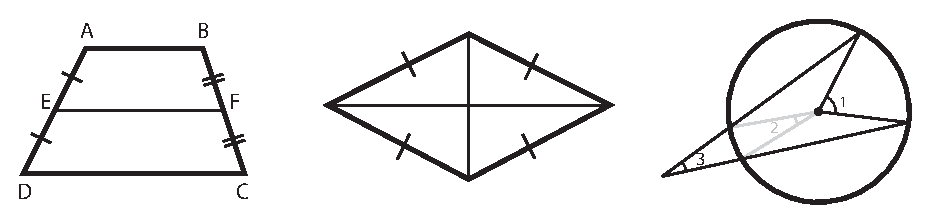
\includegraphics[width=0.95\textwidth]{diagrams/extra-diagrams.eps}
\end{center}

\noindent {\bf Investigation 3: What is interesting about the
  relationship between $AB$, $CD$, and $EF$ in the trapezoid? What is
  interesting about the diagonals of a rhombus? What is interesting
  about $\angle 1$, $\angle 2$, and $\angle 3$?}

\subsection{Nine Point Circle and Euler Segment}

Finally, this technique can be used to explore and discover
conjectures well beyond the scope of what one can visualize in his or
her head:

\begin{center}
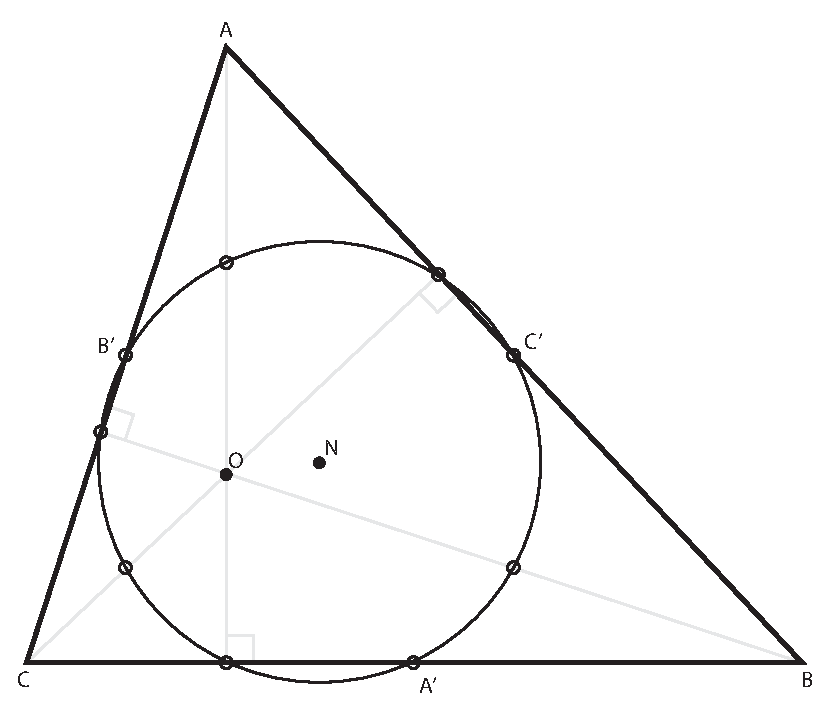
\includegraphics[width=0.6\textwidth]{diagrams/nine-point.eps}
\end{center}

\noindent {\bf Investigation 4a: In triangle $ABC$, construct the side
  midpoints $A'$, $B'$, $C'$, and orthocenter $O$ (from altitudes).
  Then, construct the midpoints of the segments connecting the
  orthocenter with each triangle vertex.  Notice anything
  interesting?}

As a more complicated example, consider the extended investigation of
the Nine Point Circle and Euler Segment.  As shown in Investigation
4a, the nine points created (feet of the altitudes, midpoints of
sides, and midpoints of segments from orthocenter to vertices) are all
concentric, lying on a circle with center labeled $N$.

Upon first constructing this figure, this fact seems almost beyond
chance.  However, as shown in Investigation 4b (below), further
``interesting properties'' continue to appear as one constructs the
centroid and circumcenter: All four of these special points ($O$, $N$,
$D$, and $M$) are collinear on what is called the \emph{Euler
  Segment}, and the ratios $ON:ND:DM$ of $3:1:2$ hold for any
triangle.

\begin{center}
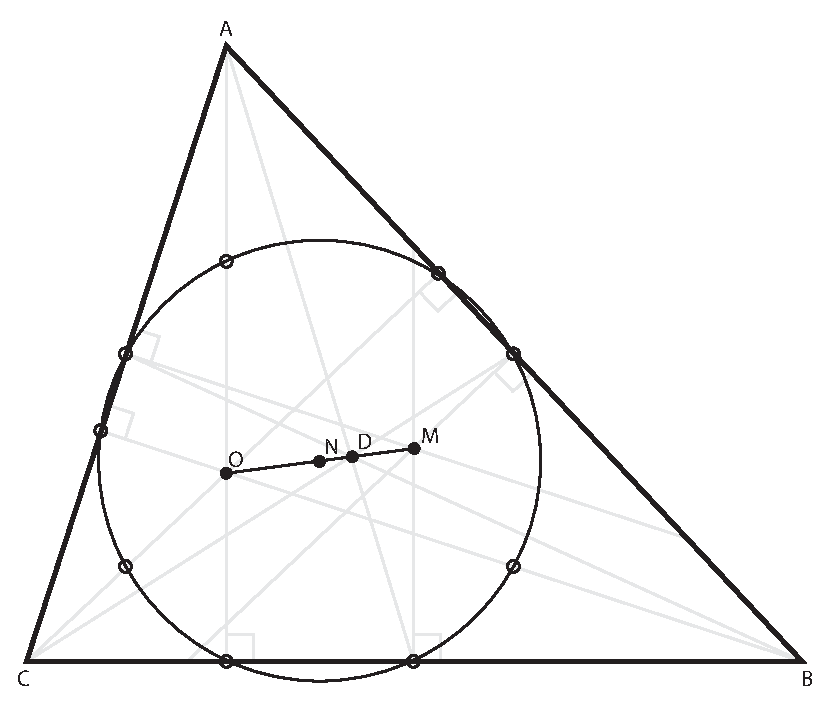
\includegraphics[width=0.7\textwidth]{diagrams/euler-line.eps}
\end{center}

\noindent {\bf Investigation 4b: Continue the investigation from 4a by
  also constructing the centroid $D$ (from medians) and circumcenter
  $M$ (from perpendicular bisectors).  Notice anything interesting?  }
